\chapter{Especificação}

\label{CapSpecs}

% Resumo opcional. Comentar se não usar.
%\resumodocapitulo{Resumo opcional}

    {O projeto \textit{RISC-V SiMPLE (Single-cycle Multicycle Pipeline Learning Environment)} consiste no desenvolvimento de um processador com conjunto de instruções \textit{RISC-V}, sintetizável em \textit{FPGA} e com \textit{hardware} descrito em \textit{Verilog}. A microarquitetura implementada nesse trabalho é uniciclo, escalar, em ordem, com um único \textit{hart} e com caminho de dados de 64 bits. Trabalhos futuros utilizarão a estrutura altamente configurável e modularizada do projeto para desenvolver as versões em microarquiteturas multiciclo e \textit{pipeline}.}

    {O processador contém o conjunto de instruções I (para operações com inteiros, sendo o único módulo com implementação mandatória pela arquitetura) e as extensões \textit{standard} M (para multiplicação e divisão de inteiros) e F (para ponto flutuante com precisão simples conforme o padrão IEEE 754 com revisão de 2008). O projeto não implementa as extensões D (ponto-flutuante de precisão dupla) e A (operações atômicas de sincronização), e com isso o \textit{soft core} desenvolvido não pode ser definido como de propósito geral, G (que deve conter os módulos I, M, A, F e D). Assim, pela nomenclatura da arquitetura, o processador desenvolvido é um \textit{RV64IMF}.}

    {O projeto contempla \textit{traps}, interrupções, exceções, \textit{CSRs}, chamadas de sistema e outras funcionalidades de nível privilegiado da arquitetura.}

    {O \textit{soft core} possui barramento Avalon para se comunicar com os periféricos das plataformas de desenvolvimento. O projeto foi desenvolvido utilizando a placa DE2-115 com \textit{FPGA Altera Cyclone} e permite a fácil adaptação para outras placas da Altera.}


    \section{Conjunto de Instruções I}
        {}

        \begin{figure}[H]
        \centering
            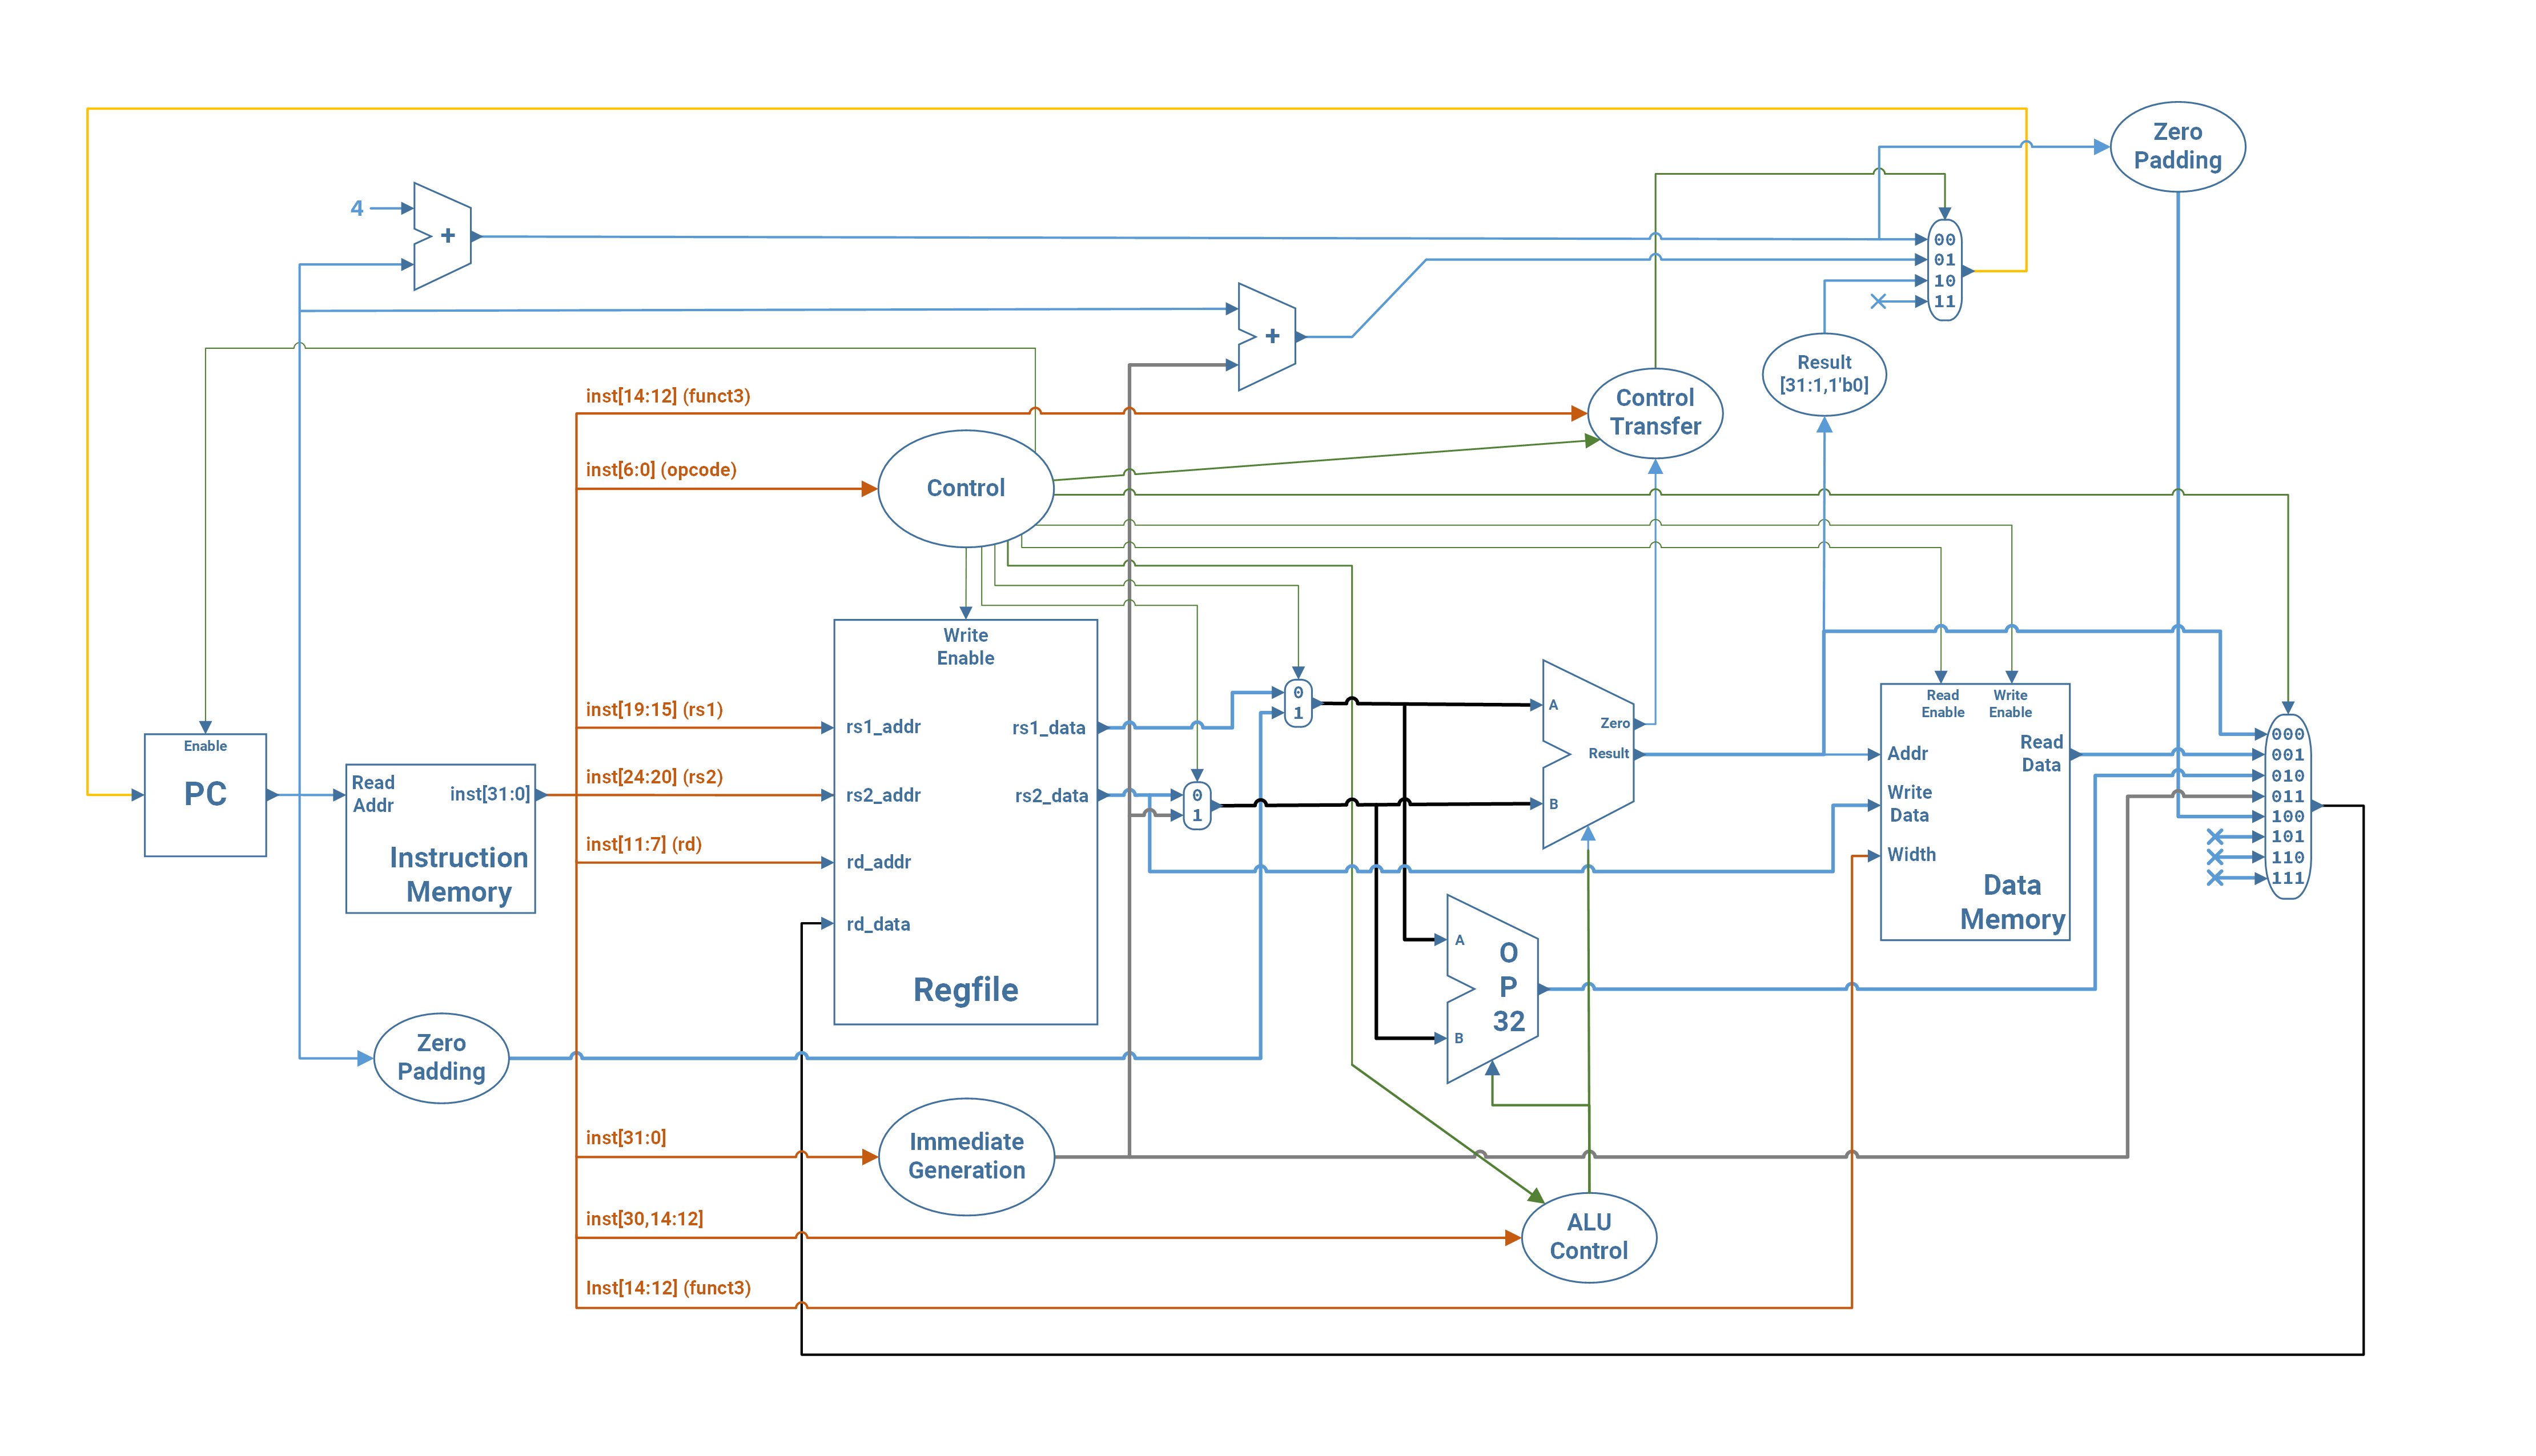
\includegraphics[width=.8\linewidth]{figs/singlecycle.png}
            \caption{Diagrama da microarquitetura uniciclo do RISC-V SiMPLE.}
            \label{fig:singlecycle}
        \end{figure}

    \section{Extensão M}
        {}

    \section{Extensão F}
        {}

    \section{Barramento Avalon}
        {}

    \section{Arquitetura Privilegiada}
        {}
